\documentclass[11pt]{article}

\usepackage{graphicx}													
\usepackage{amssymb, amsmath, amsthm} 
\usepackage{epstopdf}				%converts to pdf file
\usepackage{mathrsfs}				%something for fonts
\usepackage{xfrac}					%to make slanted fractions \sfrac{numerator}{denominator}
%\usepackage{tabu}					%to make tables in math mode $ \begin{tabular}{cccc} stuff \end{tabular} $
%\usepackage{color}					%to change font color and background color
%\usepackage[usenames,dvipsnames]{xcolor}   %to change font color to nonstandard colors
%\usepackage{colortbl}				%to add color to tables
%\usepackage{multicol}				%to add multiple columns to your document
%\usepackage{bbm}					%use \mathbbm{letter} to get letters/# that look like Naturals, etc. 
%\usepackage{hyperref} 				%to insert url's
%\usepackage{setspace}				%for spacing \doublespacing in preamble
%\usepackage{mathtools}				%to have stacked limits in sums, limits, products
									%	\sum_{\mathclap{\substack{top \\ bottom \\ another}}}
%\usepackage{caption}               %use in conjuction with subfig package
%\usepackage{subcaption}	
%\usepackage{subfig}                %mult figures with one caption, thesis file has examples
%\usepackage{enumitem}              %remove space before/after items: \begin{enumerate}[nolistsep,noitemsep]
\usepackage{tikz}                  %inline graphic \newcommand{\command}{\includegraphics[scale=0.09]{44pxtall.pdf}} 
                                    %works in and out of math mode
%\usepackage{comment}                %\begin{comment} stuff 
%\usepackage{nopageno}              %remove page number on bottom
\usepackage{fancyhdr}              %add a header
%\usepackage{showframe}             %show messed up margins
%\usepackage[margin=0.5in]{geometry} %note margins
%\usepackage[margin=1in]{geometry}   %hw margins
%\usepackage{listings}              %to display code \begin{lstlisting} code \end{lstlisting}

\renewenvironment{proof}{{\bfseries Proof}}{\qed}

\makeatletter
\renewenvironment{proof}[1][\bfseries \proofname]{\par
  \pushQED{\qed}%
  \normalfont \topsep6\p@\@plus6\p@\relax
  \trivlist
  %\itemindent\normalparindent
  \item[\hskip\labelsep
        \scshape
    #1\@addpunct{}]\ignorespaces
}{%
  \popQED\endtrivlist\@endpefalse
}
\makeatother

\newtheorem{theorem}{}
%\newtheorem{algorithm}[theorem]{Algorithm}
%\newtheorem{conjecture}[theorem]{Conjecture}
%\newtheorem{corollary}[theorem]{Corollary}
%\newtheorem{definition}[theorem]{Definition}
%\newtheorem{example}[theorem]{Example}
%\newtheorem{lemma}[theorem]{Lemma}
%\newtheorem{notation}[theorem]{Notation}
%\newtheorem{problem}[theorem]{Problem}
%\newtheorem{proposition}[theorem]{Proposition}
%\newtheorem{remark}[theorem]{Remark}
%\newtheorem{claim}[theorem]{Claim}
%\newtheorem{problemstatement}[theorem]{Problem Statement}

\newcommand{\ds}{\displaystyle}

\newcommand{\N}{\mathbb{N}}
\newcommand{\Z}{\mathbb{Z}}
\newcommand{\R}{\mathbb{R}}
\newcommand{\tA}{\tilde{\langle A \rangle}}
\newcommand{\A}{\langle A \rangle}
\newcommand{\comma}{\text{,}}
\newcommand{\period}{\text{.}}
\newcommand{\ts}{\textsuperscript}
\renewcommand\qedsymbol{$\blacksquare$}

\newcommand{\glambda}{\{G_\lambda\}_{\lambda \in A}}

%note header
%\pagestyle{fancy}
%\fancyhf{}
%\fancyhead[R]{\textcolor{white}{Q}\\ \textcolor{TealBlue}{date $\circ$ Page \thepage}}
%\renewcommand{\headrulewidth}{0pt}


% set space between paragraphs & indent if not predefined
%\parskip = 0.1in
%\parindent = 0.0in

\pagestyle{fancy}
\lhead{Trevor Klar}
\chead{July 22, 2017} 
\rhead{PUMP 2017}

\begin{document}
	
\begin{theorem} 
\textbf{Heine-Borel Theorem.} A set $E \subset \R$ is compact iff $E$ is closed and bounded.
\end{theorem}

\begin{proof} \textbf{(converse direction)}
Suppose $E$ is closed and bounded. We will show that $E$ is compact; that is, every open cover of $E$ has a finite subcover. Let $\glambda$ be an arbitrary open cover of $E$. To show that $\glambda$ has a finite subcover of of $E$, we will assume that $\glambda$ does not have a finite subcover of of $E$; and show that this assumption is self-contradictory. 

Since $E$ is bounded, there is a closed interval $[\alpha, \beta]$ which covers $E$. Let $\gamma_0$ be the midpoint of $[\alpha, \beta]$. Since $E$ cannot be covered by a finite subfamily of $\glambda$, then either $$[\alpha, \gamma_0] \cap E \text{ or } [\gamma_0, \beta] \cap E$$ cannot be covered by a finite subfamily of $\glambda$. Choose one and call it $[\alpha_1, \beta_1]$, and call $\gamma_1$ the midpoint of $[\alpha_1, \beta_1]$. Now again, either $[\alpha_1, \gamma_1] \cap E$ or $[\gamma_1, \beta_1] \cap E$ cannot be covered by a finite subfamily of $\glambda$. Choose one and call it $[\alpha_2, \beta_2]$. Continuing in this fashion, we obtain a sequence of closed intervals $[\alpha_n, \beta_n]$ with the following properties:
\begin{enumerate}
	\item $\beta_n - \alpha_n = \frac{1}{2^n}(\beta - \alpha)$. (The length of each interval is half the length of the previous interval)
	\item $[\alpha_{n+1}, \beta_{n+1}] \subset [\alpha_{n}, \beta_{n}]$ for all $n$. (This is a sequence of nested intervals)
	\item Every set $[\alpha_{n}, \beta_{n}] \cap E$ cannot be covered by a finite subfamily of $\glambda$.
\end{enumerate}
%
\begin{figure}

\end{figure}
%
By (3), $[\alpha_{n}, \beta_{n}] \cap E$  is nonempty for each $n = 1,2, \ldots \,$ ; so we may choose an element of each of these sets. Consider the set $$P = \{x_n: x_n \in [\alpha_{n}, \beta_{n}] \cap E \}.$$
There are only two possibilities: either $P$ is finite or it is infinite. We will consider each case seperately.

\textit{Case I (P is finite):} If $P$ is finite then by (2), there is an $x_{n_0} \in P$ such that, for every $[\alpha_{n}, \beta_{n}]$, 
$$ x_{n_0} \in [\alpha_{n}, \beta_{n}] \cap E.$$
Since $\glambda$ is an open cover of $E$, there is some $\lambda_0 \in A$ such that 
$$ x_{n_0} \in G_{\lambda_0}.$$
Also, since $G_{\lambda_0}$ is open, there is $\epsilon > 0$ such that 
$$(x_{n_0} - \epsilon, x_{n_0} + \epsilon) \subset G_{\lambda_0}.$$
We now have a single element of $\glambda$ which covers a neighborhood of $x_{n_0}$. We will proceed to show that this neighborhood covers one of the "uncoverable" sets $[\alpha_{n}, \beta_{n}] \cap E$ from (3).

\noindent Since $\beta_n - \alpha_n = \frac{1}{2n}(\beta - \alpha)$ for all $n$ by (1), choose $N$ large enough that 
$$\beta_N - \alpha_N = \frac{1}{2^N}(\beta - \alpha) < \epsilon.$$
So, we have that the length of $[\alpha_N, \beta_N]$ is less than $\epsilon$, and $x_{n_0} \in [\alpha_N, \beta_N]$.
So, $$x_{n_0} \leq \beta_N < x_{n_0} + \epsilon $$
and $$x_{n_0} - \epsilon < \alpha_N \leq x_{n_0}.$$
Therefore, $(x_{n_0} - \epsilon, x_{n_0} + \epsilon)$ covers $[\alpha_N, \beta_N]$, which contradicts (3).

\textit{Case II (P is infinite):} Suppose $P$ is infinite. Since $P \subset E$ and $E$ is bounded, $P$ is an infinite bounded set, which means it has an accumulation point. Call this $x_0$. Since $x_0$ is an accumulation point of $P$, $P \subset E$, and $E$ is closed; then $x_0$ is an accumulation point of $E$ and $x_0 \in E$. Since $\glambda$ covers E, there is a $\lambda_1 \in A$ such that $x_0 \in G_{\lambda_1}$; and since $G_{\lambda_1}$ is open, there is $\epsilon > 0$ such that 
$$x_0 \in (x_0 - \epsilon, x_0 + \epsilon) \subset G_{\lambda_1}.$$
We will now show that this neighborhood of $x_0$ covers one of the "uncoverable" intervals. By the same reasoning in Case I, choose $N$ large enough that 
$$\beta_N - \alpha_N < \frac{\epsilon}{2}.$$
Since $x_0$ is an accumulation point of P, there are infinitely many elements of $P$ in each neighborhood of $x_0$, so we can find an $M > N$ such that 
$$|x_0 - x_M| < \frac{\epsilon}{2}.$$
Now, since $M>N$, then $[\alpha_M, \beta_M] \subset [\alpha_N, \beta_N]$, so  
$$\beta_M - \alpha_M < \beta_N - \alpha_N < \frac{\epsilon}{2}.$$
This means that since $x_M \in [\alpha_M, \beta_M]$, we now have that for any $x \in [\alpha_M, \beta_M]$, 
$$ |x_M - x|< \frac{\epsilon}{2}.$$
Recall that by (3), no finite subfamily of $\glambda$ covers $[\alpha_M, \beta_M]$. However, for any $x \in [\alpha_M, \beta_M]$,

\begin{center}
\begin{tabular}{rcl}
$|x_0 - x|$ 	& $=$	& $|x_0 - x_M + x_M - x|$ \\
				& $\leq$	& $|x_0 - x_M| + |x_M - x|$  \\
				& $<$	& $\dfrac{\epsilon}{2} + \dfrac{\epsilon}{2}$  \\
				& $<$	& $\epsilon.$  \\
\end{tabular}
\end{center}
Therefore, $(x_0 - \epsilon, x_0 + \epsilon) \subset G_{\lambda_1}$ covers $[\alpha_M, \beta_M]$, which is a contradiction.

Thus, we have shown that $\glambda$, an arbitrary open cover of $E$, must necessarily have a finite subcover of $E$, so $E$ is compact.  
\end{proof}

\begin{proof} \textbf{(forward direction)}
Suppose $E$ is compact. We will show that $E$ is closed and bounded by contrapositive; that is, if $E$ is either not closed or not bounded, then $E$ is not compact.

\textit{Case I ($E$ is not bounded):} Assume $E$ is not bounded. To show that $E$ is not compact, we will produce an open cover of $E$ which has no finite subcover. Let $\{G_n\}_{n=1}^{\infty}$ be the collection of all open intervals 
$$G_n = (-n,n).$$ 
Now, $\{G_n\}_{n=1}^{\infty}$ is an open cover of $\R$, so it certainly covers $E$. To specify an arbitrary subcover of $\{G_n\}_{n=1}^{\infty}$; let $S \subset \N$ be some finite set of positive integers. Since, for any $n<m$, $G_n \subset G_m$, then 
$$\bigcup_{n \in S} G_n = G_{max(S)}.$$  
However, since $E$ is unbounded, $E \not\subset G_{max(S)}$. Thus, $\{G_n\}_{n=1}^{\infty}$ is an open cover of $E$ with no finite subcover, so $E$ is not compact. 

\textit{Case II ($E$ is not closed):} Assume $E$ is not closed. Then there is an accumulation point of $E$ (call it $x_0$) such that $x_0 \not\in E$. For each positive integer $n$, define
$$G_n = \left(-\infty, x_0-\tfrac{1}{n}\right) \cup \left(x_0+\tfrac{1}{n}, \infty\right).$$
Note that $\{G_n\}_{n=1}^{\infty}$ covers $\R \setminus \{x_0\}$, so it also covers $E$. We will again specify an arbitrary subcover of $\{G_n\}_{n=1}^{\infty}$ by letting $S \subset \N$ be some finite set of positive integers; and noting again that, for any $n<m$, $G_n \subset G_m$, so 
$$\bigcup_{n \in S} G_n = G_{max(S)}.$$
Let $N = max(S)$. Then, $\bigcup_{n \in S} G_n  = G_N = \left(-\infty, x_0-\sfrac{1}{N}\right) \cup \left(x_0+\sfrac{1}{N}, \infty\right).$ However, since $x_0$ is an accumulation point of $E$, $(x_0-\sfrac{1}{N} , x_0+\sfrac{1}{N})$ contains infinitely many elements of $E$, none of which are in $G_N$. Therefore, $\{G_n\}_{n=1}^{\infty}$ has no finite subcover of $E$, so $E$ is not compact. 
\end{proof}

\newpage
\begin{center}
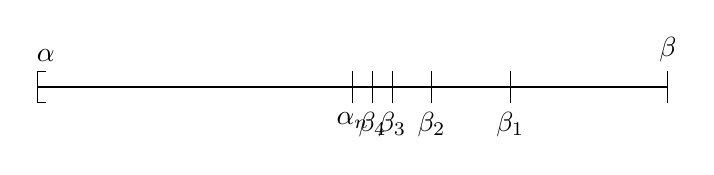
\begin{tikzpicture}[scale=4]
%[-1,1]
%[0,1]
%[0,1/2^(n-1)]

\draw (-1,0) -- (1,0);
\draw (-1+.025,-.05) -- (-1,-.05) -- (-1,.05) -- (-1+.025,.05) node[anchor=south] {$\alpha$};
\draw (1,-.05) -- (1,.05) node[anchor=south] {$\beta$};
\draw (0,.05) -- (0,-.05) node[anchor=north] {$\alpha_n$};
\foreach \n in {1,2,3,4}
  {\draw (1/2^\n,.05) -- (1/2^\n,-.05) node[anchor=north] {$\beta_{\n}$};}

\end{tikzpicture}
\end{center}


\begin{center}
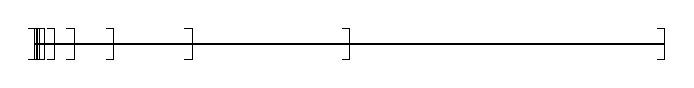
\begin{tikzpicture}[scale=4]
\draw (-1,0) -- (1,0);
\draw (-1+.025,-.05) -- (-1,-.05) -- (-1,.05) -- (-1+.025,.05);
\draw (-1+.025,-.05) -- (-1,-.05) -- (-1,.05) -- (-1+.025,.05);
\draw (-1+.025,-.05) -- (-1,-.05) -- (-1,.05) -- (-1+.025,.05);
\draw (-1+.025,-.05) -- (-1,-.05) -- (-1,.05) -- (-1+.025,.05);
\draw (-1+.025,-.05) -- (-1,-.05) -- (-1,.05) -- (-1+.025,.05);
\draw (-1+.025,-.05) -- (-1,-.05) -- (-1,.05) -- (-1+.025,.05);
\draw (-1+.025,-.05) -- (-1,-.05) -- (-1,.05) -- (-1+.025,.05);
\draw (-1+.025,-.05) -- (-1,-.05) -- (-1,.05) -- (-1+.025,.05);
\draw (-1+.025,-.05) -- (-1,-.05) -- (-1,.05) -- (-1+.025,.05);
\draw (-1+.025,-.05) -- (-1,-.05) -- (-1,.05) -- (-1+.025,.05);
\draw (1-.025,-.05) -- (1,-.05) -- (1,.05) -- (1-.025,.05);
\draw (0.0-.025,-.05) -- (0.0,-.05) -- (0.0,.05) -- (0.0-.025,.05);
\draw (-0.5-.025,-.05) -- (-0.5,-.05) -- (-0.5,.05) -- (-0.5-.025,.05);
\draw (-0.75-.025,-.05) -- (-0.75,-.05) -- (-0.75,.05) -- (-0.75-.025,.05);
\draw (-0.875-.025,-.05) -- (-0.875,-.05) -- (-0.875,.05) -- (-0.875-.025,.05);
\draw (-0.9375-.025,-.05) -- (-0.9375,-.05) -- (-0.9375,.05) -- (-0.9375-.025,.05);
\draw (-0.96875-.025,-.05) -- (-0.96875,-.05) -- (-0.96875,.05) -- (-0.96875-.025,.05);
\draw (-0.984375-.025,-.05) -- (-0.984375,-.05) -- (-0.984375,.05) -- (-0.984375-.025,.05);
\draw (-0.9921875-.025,-.05) -- (-0.9921875,-.05) -- (-0.9921875,.05) -- (-0.9921875-.025,.05);
\draw (-0.99609375-.025,-.05) -- (-0.99609375,-.05) -- (-0.99609375,.05) -- (-0.99609375-.025,.05);
\end{tikzpicture}
\end{center}

\begin{center}
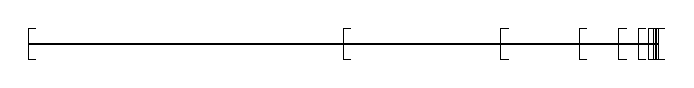
\begin{tikzpicture}[scale=4]
\draw (-1,0) -- (1,0);
\draw (-1+.025,-.05) -- (-1,-.05) -- (-1,.05) -- (-1+.025,.05);
\draw (0.0+.025,-.05) -- (0.0,-.05) -- (0.0,.05) -- (0.0+.025,.05);
\draw (0.5+.025,-.05) -- (0.5,-.05) -- (0.5,.05) -- (0.5+.025,.05);
\draw (0.75+.025,-.05) -- (0.75,-.05) -- (0.75,.05) -- (0.75+.025,.05);
\draw (0.875+.025,-.05) -- (0.875,-.05) -- (0.875,.05) -- (0.875+.025,.05);
\draw (0.9375+.025,-.05) -- (0.9375,-.05) -- (0.9375,.05) -- (0.9375+.025,.05);
\draw (0.96875+.025,-.05) -- (0.96875,-.05) -- (0.96875,.05) -- (0.96875+.025,.05);
\draw (0.984375+.025,-.05) -- (0.984375,-.05) -- (0.984375,.05) -- (0.984375+.025,.05);
\draw (0.9921875+.025,-.05) -- (0.9921875,-.05) -- (0.9921875,.05) -- (0.9921875+.025,.05);
\draw (0.99609375+.025,-.05) -- (0.99609375,-.05) -- (0.99609375,.05) -- (0.99609375+.025,.05);
\draw (1-.025,-.05) -- (1,-.05) -- (1,.05) -- (1-.025,.05);
\draw (1-.025,-.05) -- (1,-.05) -- (1,.05) -- (1-.025,.05);
\draw (1-.025,-.05) -- (1,-.05) -- (1,.05) -- (1-.025,.05);
\draw (1-.025,-.05) -- (1,-.05) -- (1,.05) -- (1-.025,.05);
\draw (1-.025,-.05) -- (1,-.05) -- (1,.05) -- (1-.025,.05);
\draw (1-.025,-.05) -- (1,-.05) -- (1,.05) -- (1-.025,.05);
\draw (1-.025,-.05) -- (1,-.05) -- (1,.05) -- (1-.025,.05);
\draw (1-.025,-.05) -- (1,-.05) -- (1,.05) -- (1-.025,.05);
\draw (1-.025,-.05) -- (1,-.05) -- (1,.05) -- (1-.025,.05);
\draw (1-.025,-.05) -- (1,-.05) -- (1,.05) -- (1-.025,.05);
\end{tikzpicture}
\end{center}

\begin{center}
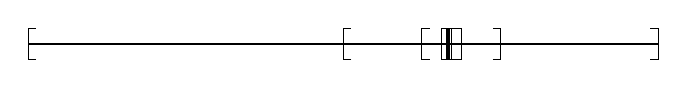
\begin{tikzpicture}[scale=4]
\draw (-1,0) -- (1,0);
\draw (-1+.025,-.05) -- (-1,-.05) -- (-1,.05) -- (-1+.025,.05);
\draw (0.0+.025,-.05) -- (0.0,-.05) -- (0.0,.05) -- (0.0+.025,.05);
\draw (0.0+.025,-.05) -- (0.0,-.05) -- (0.0,.05) -- (0.0+.025,.05);
\draw (0.25+.025,-.05) -- (0.25,-.05) -- (0.25,.05) -- (0.25+.025,.05);
\draw (0.25+.025,-.05) -- (0.25,-.05) -- (0.25,.05) -- (0.25+.025,.05);
\draw (0.3125+.025,-.05) -- (0.3125,-.05) -- (0.3125,.05) -- (0.3125+.025,.05);
\draw (0.3125+.025,-.05) -- (0.3125,-.05) -- (0.3125,.05) -- (0.3125+.025,.05);
\draw (0.328125+.025,-.05) -- (0.328125,-.05) -- (0.328125,.05) -- (0.328125+.025,.05);
\draw (0.328125+.025,-.05) -- (0.328125,-.05) -- (0.328125,.05) -- (0.328125+.025,.05);
\draw (0.33203125+.025,-.05) -- (0.33203125,-.05) -- (0.33203125,.05) -- (0.33203125+.025,.05);
\draw (1-.025,-.05) -- (1,-.05) -- (1,.05) -- (1-.025,.05);
\draw (1-.025,-.05) -- (1,-.05) -- (1,.05) -- (1-.025,.05);
\draw (0.5-.025,-.05) -- (0.5,-.05) -- (0.5,.05) -- (0.5-.025,.05);
\draw (0.5-.025,-.05) -- (0.5,-.05) -- (0.5,.05) -- (0.5-.025,.05);
\draw (0.375-.025,-.05) -- (0.375,-.05) -- (0.375,.05) -- (0.375-.025,.05);
\draw (0.375-.025,-.05) -- (0.375,-.05) -- (0.375,.05) -- (0.375-.025,.05);
\draw (0.34375-.025,-.05) -- (0.34375,-.05) -- (0.34375,.05) -- (0.34375-.025,.05);
\draw (0.34375-.025,-.05) -- (0.34375,-.05) -- (0.34375,.05) -- (0.34375-.025,.05);
\draw (0.3359375-.025,-.05) -- (0.3359375,-.05) -- (0.3359375,.05) -- (0.3359375-.025,.05);
\draw (0.3359375-.025,-.05) -- (0.3359375,-.05) -- (0.3359375,.05) -- (0.3359375-.025,.05);
\end{tikzpicture}
\end{center}

\begin{center}
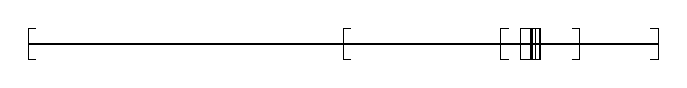
\begin{tikzpicture}[scale=4]
\draw (-1,0) -- (1,0);
\draw (-1+.025,-.05) -- (-1,-.05) -- (-1,.05) -- (-1+.025,.05);
\draw (0.0+.025,-.05) -- (0.0,-.05) -- (0.0,.05) -- (0.0+.025,.05);
\draw (0.5+.025,-.05) -- (0.5,-.05) -- (0.5,.05) -- (0.5+.025,.05);
\draw (0.5+.025,-.05) -- (0.5,-.05) -- (0.5,.05) -- (0.5+.025,.05);
\draw (0.5+.025,-.05) -- (0.5,-.05) -- (0.5,.05) -- (0.5+.025,.05);
\draw (0.5625+.025,-.05) -- (0.5625,-.05) -- (0.5625,.05) -- (0.5625+.025,.05);
\draw (0.59375+.025,-.05) -- (0.59375,-.05) -- (0.59375,.05) -- (0.59375+.025,.05);
\draw (0.59375+.025,-.05) -- (0.59375,-.05) -- (0.59375,.05) -- (0.59375+.025,.05);
\draw (0.59375+.025,-.05) -- (0.59375,-.05) -- (0.59375,.05) -- (0.59375+.025,.05);
\draw (0.59375+.025,-.05) -- (0.59375,-.05) -- (0.59375,.05) -- (0.59375+.025,.05);
\draw (1-.025,-.05) -- (1,-.05) -- (1,.05) -- (1-.025,.05);
\draw (1-.025,-.05) -- (1,-.05) -- (1,.05) -- (1-.025,.05);
\draw (1-.025,-.05) -- (1,-.05) -- (1,.05) -- (1-.025,.05);
\draw (0.75-.025,-.05) -- (0.75,-.05) -- (0.75,.05) -- (0.75-.025,.05);
\draw (0.625-.025,-.05) -- (0.625,-.05) -- (0.625,.05) -- (0.625-.025,.05);
\draw (0.625-.025,-.05) -- (0.625,-.05) -- (0.625,.05) -- (0.625-.025,.05);
\draw (0.625-.025,-.05) -- (0.625,-.05) -- (0.625,.05) -- (0.625-.025,.05);
\draw (0.609375-.025,-.05) -- (0.609375,-.05) -- (0.609375,.05) -- (0.609375-.025,.05);
\draw (0.6015625-.025,-.05) -- (0.6015625,-.05) -- (0.6015625,.05) -- (0.6015625-.025,.05);
\draw (0.59765625-.025,-.05) -- (0.59765625,-.05) -- (0.59765625,.05) -- (0.59765625-.025,.05);
\end{tikzpicture}
\end{center}

\begin{tikzpicture}[xscale=25,yscale=5]
\draw [<->, help lines] (0.6,1.34) -- (0.6,1) -- (1.05,1);
\draw[orange] (0.6, 1.0385) --
(0.61, 1.06372) -- (0.62, 1.08756) -- (0.63, 1.11012) -- (0.64,
1.13147) -- (0.65, 1.15166) -- (0.66, 1.17074) -- (0.67, 1.18874) -- (0.68,
1.20568) -- (0.69, 1.22157) -- (0.7, 1.23643) -- (0.71, 1.25026) -- (0.72,
1.26307) -- (0.73, 1.27486) -- (0.74, 1.28561) -- (0.75, 1.29534) -- (0.76,
1.30402) -- (0.77, 1.31165) -- (0.78, 1.31821) -- (0.79, 1.32369) -- (0.8,
1.32806) -- (0.81, 1.33131) -- (0.82, 1.3334) -- (0.83, 1.33431) -- (0.84,
1.334) -- (0.85, 1.33244) -- (0.86, 1.32956) -- (0.87, 1.32533) -- (0.88,
1.31966) -- (0.89, 1.3125) -- (0.9, 1.30373) -- (0.91, 1.29325) -- (0.92,
1.2809) -- (0.93, 1.26649) -- (0.94, 1.24976) -- (0.95, 1.23032) -- (0.96,
1.2076) -- (0.97, 1.18065) -- (0.98, 1.14763) -- (0.99, 1.1038) -- (0.991,
1.09836) -- (0.992, 1.09261) -- (0.993, 1.0865) -- (0.994, 1.07994) -- (0.995,
1.07282) -- (0.996, 1.06497) -- (0.997, 1.0561) -- (0.998, 1.04563) -- (0.999,
1.03209) -- (0.9991, 1.03042) -- (0.9992, 1.02866) -- (0.9993,
1.02679) -- (0.9994, 1.02478) -- (0.9995, 1.0226) -- (0.9996, 1.02019) -- (0.9997,
1.01747) -- (0.9998, 1.01424) -- (0.9999, 1.01005) -- (0.9999,
1.01005) -- (0.99991, 1.00953) -- (0.99992, 1.00898) -- (0.99993,
1.0084) -- (0.99994, 1.00778) -- (0.99995, 1.0071) -- (0.99996,
1.00634) -- (0.99997, 1.00549) -- (0.99998, 1.00448) -- (0.99999, 1.00317) -- (1,
1) ;
\end{tikzpicture}


\end{document}


%\begin{equation*}
%	y =  \left\{
%		\begin{aligned}
%			line 1 \\
%			line 2
%		\end{aligned}
%	\right.
%\end{equation*}

%\begin{center} \includegraphics[width=0.4\linewidth]{prob1.jpg} \end{center}

